\documentclass{article}

\usepackage[accepted]{icml2023}

% Packages
\usepackage{hyperref}
\usepackage{graphicx}
\usepackage{booktabs}
\usepackage{multirow}
\usepackage{amsmath}
\usepackage{xcolor}
\usepackage{subcaption}
\usepackage{listings}
\usepackage{float}

% Aliases
\newcommand{\github}{\href{https://github.com/mikasenghaas/swarm}{GitHub}}
\newcommand{\wandb}{\href{https://wandb.ai/mikasenghaas/swarm}{Weights \& Biases}}
\newcommand{\gist}{\href{https://gist.github.com/mikasenghaas/5fa1aa77ea69f187f531a5889983c249}{GitHub Gist}}

% Colours
\definecolor{bblue}{HTML}{5884E2}
\definecolor{oorange}{HTML}{F19E38}

% Code
\definecolor{codegreen}{rgb}{0,0.6,0}
\definecolor{codegray}{rgb}{0.5,0.5,0.5}
\definecolor{codepurple}{rgb}{0.58,0,0.82}
\definecolor{backcolour}{rgb}{0.95,0.95,0.95}
\lstdefinestyle{mystyle}{
    backgroundcolor=\color{backcolour},   
    commentstyle=\color{codegreen},
    keywordstyle=\color{magenta},
    numberstyle=\tiny\color{codegray},
    stringstyle=\color{codepurple},
    basicstyle=\ttfamily\footnotesize,
    showspaces=false,                
    showstringspaces=false,
    showtabs=false,                  
    tabsize=2
}
\lstset{style=mystyle}

% Running Title
\icmltitlerunning{DiLoCo-SWARM}

\begin{document}

% Title
\twocolumn[
  \icmltitle{DiLoCo-SWARM}
  \begin{icmlauthorlist}
    \icmlauthor{Mika Senghaas}{author}
    \icmlauthor{Martijn De Vos}{supervisor}
    \icmlauthor{Akash Dhasad}{supervisor}
    \icmlauthor{Rishi Sharma}{supervisor}
  \end{icmlauthorlist}
  \icmlaffiliation{author}{Author}
  \icmlaffiliation{supervisor}{Supervisor}
  \icmlcorrespondingauthor{Mika Senghaas}{mika.senghaas@epfl.ch}
  \icmlkeywords{Distributed Training, Decentralized AI, SWARM, DiLoCo}
  \vskip 0.3in
]
\printAffiliationsAndNotice{}

% Abstract
\begin{abstract}
  We investigate DiLoCo-SWARM, a decentralized training approach that combines
  the pipeline and data parallelism of SWARM with DiLoCo's reduced-frequency
  gradient synchronization. Our experiments on language modeling tasks show that
  DiLoCo-SWARM matches or surpasses fully synchronized SWARM baselines despite
  synchronizing gradients up to 50 times less frequently.
\end{abstract}

\section{Introduction}

% Centralized training
Modern foundation models have billions of parameters and are trained on
trillions of
tokens~\cite{chowdhery2022palm,brown2023gpt3,dubey2024llama3,google2024gemini}.
Operating at such scale requires orchestrating thousands of GPUs to distribute
computation~\cite{dubey2024llama3,deepseekai2024}. However, traditional
parallelization techniques rely on fast interconnect to not bottleneck the
training. Hence, frontier-scale models are currently trained in high performance
clusters (HPC). Operating HPCs requires billions of dollars, leaving research
capabilities to a small number of corporate and state
entities~\cite{jaghouar2024intellect1}. 

% This creates significant points of control, and in turn increases the risk of
% capability capture or misue.

% Decentralized training
Recently, decentralization has emerged as a promising counter-weight to this
trajectory. Decentralized training aims to pool the vast, cheap compute
resources across the globe for collaborative model training. It promises smaller
actors access to large-scale compute at significantly reduced cost, with the
potential to accelerate open-source AI development.  However, this new paradigm
comes with significant technical and algorithmic challenges: nodes have to
communicate via common internet connections, leading to orders of magnitude
lower network bandwidths, and the pool of training nodes can be heterogeneous -
nodes may have varying performance - and dynamic - nodes may join or leave
training unpredictably.

% Intellect-1 and DiLoCo
Hence, current decentral training efforts can not yet match the scale and
efficiency of the centralized setting. Yet, the field is progressing rapidly and
is gaining interest in the research community.
INTELLECT-1~\cite{jaghouar2024intellect1} is the most recent demonstration that
large-scale decentral model training is possible. It is a 10B parameter model
trained across three continents. The model is a scale-up of
DiLoCo~\cite{douillard2023diloco}, a low-cost communication distributed data
parallel (DDP) training method. Compared to traditional DDP, DiLoCo's key
insight is to replace regular gradient synchronization at every step with less
frequent synchronization using an dual optimization scheme. Their empirical
results show that the method preserves performance while requiring a fraction of
the communication cost, i.e. only every 500 steps. The experiments have since
been replicated~\cite{jaghouar2024opendiloco}, and engineered further to enable
billion-parameter training runs in the form of
INTELLECT-1~\cite{jaghouar2024intellect1}.  However, a key limitation is that
each node has to store a full copy of the model to participate during training,
and that heterogeneous compute can bottlenecks compute utilization. For this
reason, the minimum requirement for a node were 8xH100 GPUs to contribute to
training INTELLECT-1.

% SWARM
SWARM~\cite{ryabinin2023swarm} parallelism is a promising, but less explored,
alternative for decentralized training that is designed for larger scale. Unlike
DiLoCo, which relies solely on data parallelism, SWARM combines two types of 
parallelism - data and pipeline paralleparallelism. By also sharding the model,
SWARM can scale to larger models, or vice versa, allow lower-end devices to
participate in training. This makes it an attractive candidate for further
scaling decentralized training efforts. In its original formulation, SWARM
requires gradient synchronization between all nodes serving the same pipeline
stage of a model. 

% DiLoCo-SWARM
The successes and robustness of DiLoCo motivates this research which
investigates whether step-wise gradient synchronization in SWARM pipeline stages
can be replaced by DiLoCo-style synchronization. We make the following two
contributions:

\begin{enumerate}
  \item \textbf{DiLoCo-SWARM.} We show that SWARM parallelism is compatible with
  DiLoCo-style gradient synchronization, allowing to train SWARM while requiring
  significantly fewer synchronization of gradients while retaining
  generalization performance.
  \item \textbf{Implementation.} We release a minimal training script
  implementing a feature subset of SWARM parallelism, as well the DiLoCo
  optimizer.  Instead of multiple thousands, the implementation uses a few
  hundred lines of pure PyTorch code.
\end{enumerate}

Besides open-sourcing the full experiment code and results on \github{} and
\wandb{}, we release a distilled version of the training logic as a \gist{}. We
hope that these resources will serve as a starting point for further open-source
research efforts with SWARM, and spark interest in scaling SWARM from research
to
production-grade systems, similarly to development of DiLoCo.

\section{Background}

\subsection{Distributed Training}

In distributed training, $n$ nodes collaboratively train a \textit{model}
$f_{\theta}$ parameterized by its weights $\theta$, on a \textit{dataset} of
samples $D = \{(\mathbf{x}_e, \mathbf{y}_1),\dots\}$. Collaboration requires
nodes to periodically communicate intermediate results. We will describe two of
the most widely used forms of parallelization, relevant in the context of
DiLoCo-SWARM.

\begin{figure}[ht]
    \centering
    \begin{subfigure}[b]{0.22\textwidth}
        \centering
        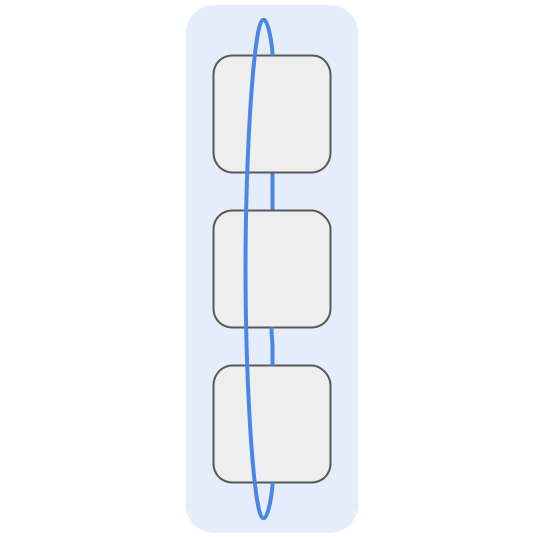
\includegraphics[width=\textwidth]{figures/dp.png}
        \caption{Data Parallelism}
    \end{subfigure}
    \hfill
    \begin{subfigure}[b]{0.22\textwidth}
        \centering
        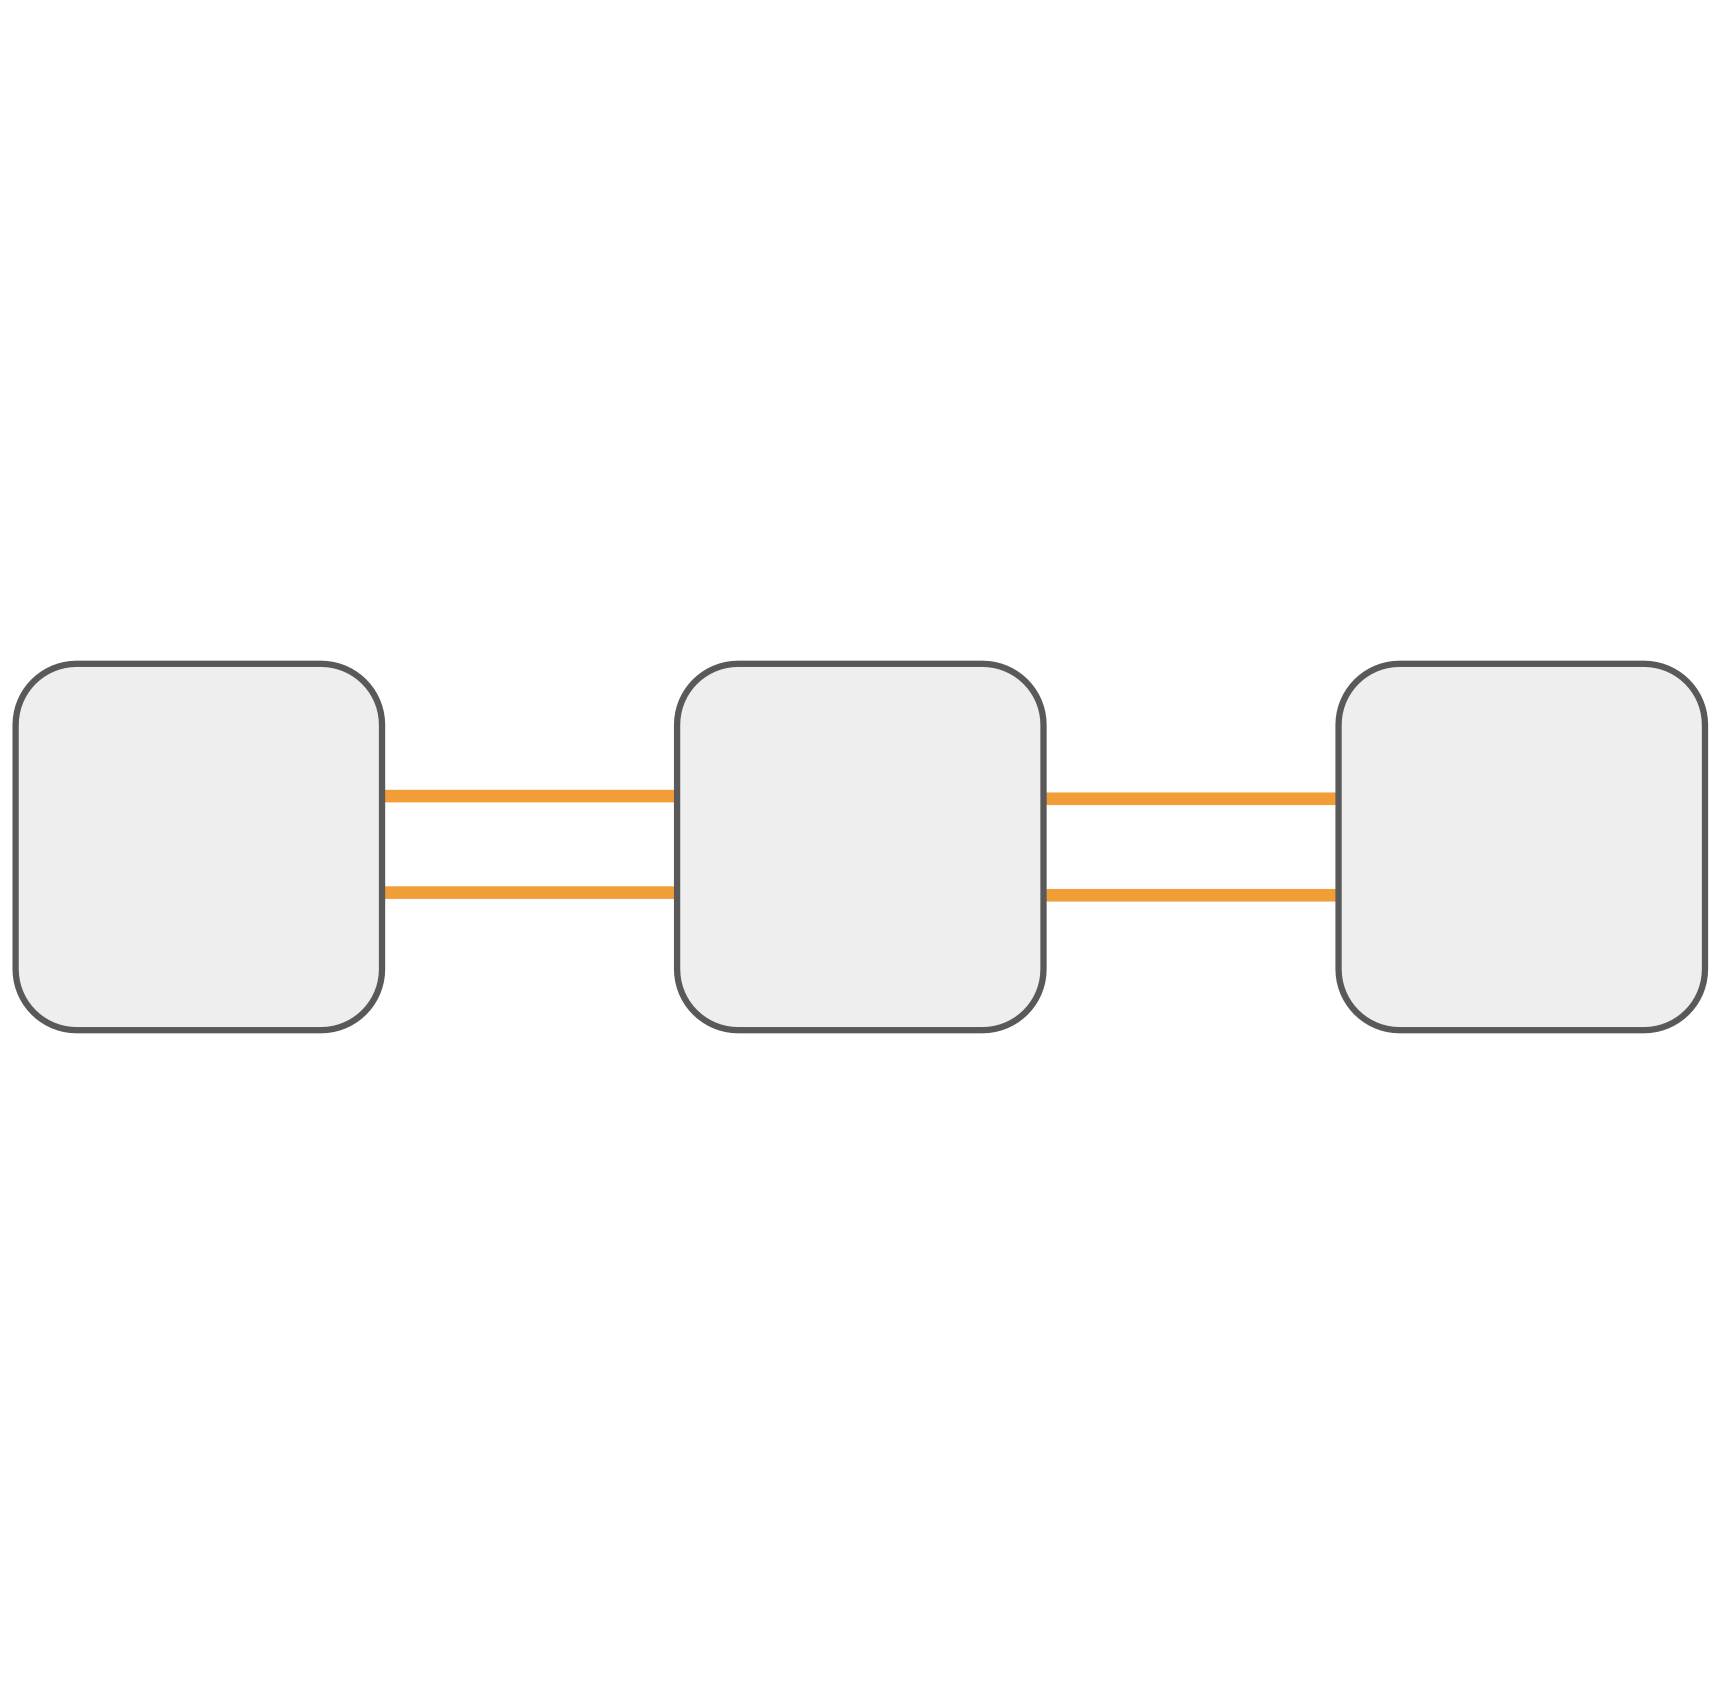
\includegraphics[width=\textwidth]{figures/pp.png}
        \caption{PP Parallelism}
    \end{subfigure}
    \caption{\textbf{DP and PP Communication} High-level visualization of DP and
    PP communication patterns for $n=3$ nodes. Nodes are represented as boxes,
    communication as links. {\color{bblue} Blue links} represent
    \texttt{AllReduce} operations to average gradients between nodes. 
    {\color{oorange}Orange links} represent bi-directional point-to-point
    communication between adjacent stages.}
    \label{fig:dp-pp}
\end{figure}

\textit{Data parallelism} (DP) partitions the dataset, creating $n$ data shards
$D_1,\dots,D_n$. The $i$-th node only holds a (local) data shard $D_i$ and a
copy of the full model parameters $\theta$. Training proceeds as shown in
Algorithm~\ref{alg:dp}: Each node samples a batch from its local data shard,
computes local gradients via a full forward and backward pass, but before
updating the model, averages the gradients from all workers via an
\texttt{AllReduce} operation. DP communication cost scales with the number of
model parameters and number of nodes.

\begin{algorithm}
\caption{Data Parallel Gradient Synchronization}
\label{alg:dp}
\begin{algorithmic}
\STATE {\bfseries Input:} Local Dataset $D_i$, Model $\theta^{(t-1)}$, Optimizer $\mathtt{OPT}$, Loss $\mathcal{L}$
\STATE Sample batch: $x_i\sim D_i$
\STATE Compute gradient: $g_i \gets \nabla_{\theta_i} \mathcal{L}(x_i; \theta^{(t-1)})$
\STATE Sync gradients: $g \gets \frac{1}{n}\sum_{i}^n g_i$ \COMMENT{$\mathtt{AllReduce}$}
\STATE Update model: $\theta_i^{(t)} \gets \mathtt{OPT}(\theta_i^{(t-1)}, g)$
\end{algorithmic}
\end{algorithm}

\textit{Pipeline parallelism} (PP) partitions the model, creating $n$ model
shards $f'$ parameterized by $\theta_1,\dots,\theta_n$, such that the full model
is reconstructed by concatenation of the shards, i.e.
$f_{\theta}=f'_{\theta_1}\circ\dots\circ f'_{\theta_n}$. Due to the sequential
dependency, shards represent "stages" in the pipeline, where the $i$-th stage
serves the model shard $f_{\theta_i}$. For most deep learning model such a
sequential partition is natural, as they are architected as repeated
computational blocks. For example, in Transformer one stage handles one or more
Transformer blocks consisting of attention and feed-forward
layers~\cite{vaswani2017transformer}. The partitioning creates a bi-directional
communication pattern between stages during training, as shown in
Figure~\ref{fig:dp-pp}: During a forward pass activations are communicated from
stage $i$ to $i+1$, and during the backward pass gradients are sent from stage
$i$ to $i-1$. Despite its simplicity, PP is notoriously hard to optimize. Naive
implementations suffer from significant GPU idle time, e.g. when the first node
has to wait for the full pipeline forward and backward pass before being able to
compute gradients. Efficient PP implementations therefore rely on micro-batching
and advanced scheduling techniques to be practically viable. PP communication
scales with the number of stages $n$ and the model's hidden dimension.

Typically, different forms of parallelism can be combined. In the case of DP and
PP, a natural combination is to partition both the dataset and model into
$\{D_i\}_{i\in [m]}$ and $\{\theta_j\}_{j\in [n]}$, respectively. This creates a
$m\times n$ grid structure, where the $(i,j)$-th node handles data shard $D_i$
and model shard $\theta_j$. During training, DP and PP communication is
interleaved: First, nodes send activations and gradients (PP communication)
within each of the $i=1\dots,m$ pipelines to accumulate local gradients. Then,
within each stage $j=1,\dots,n$, the nodes run an \texttt{AllReduce} to average
accumulated gradients for their local shard (DP communication).

\subsection{DiLoCo}

In the decentralized setting, interconnect may be slow and so regular gradient
synchronization as shown in Algorithm~\ref{alg:dp} can bottleneck the training
process, especially when scaling to larger models. Distributed Low-Cost
Communication (DiLoCo)~\cite{douillard2023diloco} is data parallel training method
which reduces the frequency at which gradients are synchronized via a dual
optimization scheme. As shown in Algorithm~\ref{alg:diloco} each node trains for
a fixed number of inner steps using a local optimizer. To synchronize with the
remaining workers, it computes and averages its pseudo-gradient (the difference
between the parameters before and after the inner optimization.) with all nodes
via \texttt{AllReduce} to update a global model using an global optimizer. 

\begin{algorithm}
\caption{DiLoCo Gradient Synchronization}
\label{alg:diloco}
\begin{algorithmic}[1]
\STATE \textbf{Input:} Local dataset $D_i$, Model $\theta^{(t-1)}$, Optimizers $\mathtt{OPT}_{\text{local}}$ and $\mathtt{OPT}_{\text{global}}$, Loss $\mathcal{L}$, Local Steps $H$ 
\STATE Copy global model: $\theta_i^{(t-1)} \gets \theta^{(t-1)}$
\FOR{$H$ steps}
  \STATE Sample batch: $x \sim D_i$
  \STATE Compute gradient: $g_i \gets \nabla_{\theta_i} \mathcal{L}(x_i; \theta_i^{(t-1)})$
  \STATE Update local model: $\theta_i^{(t-1)} \gets \mathtt{OPT}_{\text{local}}(\theta_i^{(t-1)}, g_i)$
\ENDFOR
\STATE Compute pseudo-gradient: $\Delta_i \gets \theta_i^{(t-1)} - \theta^{(t-1)}$
\STATE Sync pseudo-gradients: $\Delta \gets \frac{1}{n}\sum_i^n \Delta_i$ \COMMENT{$\mathtt{AllReduce}$}
\STATE Update global model: $\theta^{(t)} \gets \mathtt{OPT}_{\text{global}}(\theta^{(t-1)}, \Delta)$
\end{algorithmic}
\end{algorithm}

Empirical results show that DiLoCo drastically reduces the frequency at which
gradients need to be synchronized. Despite only synchronizing every $500$ local
steps, they can match the generalization performance of a DP baseline. However,
DiLoCo shares many challenges with traditional data parallel training. Most
notably, DiLoCo does not scale naturally to models that do not fit into the
local workers' memory - relying on slow parameter offloading
methods~\cite{rhu2016, cui2016}, gradient quantization~\cite{jaghouar2024intellect1} and
other tricks for scaling, which come at the cost of reduced efficiency for
scaling, which come at the cost of reduced efficiency

\subsection{SWARM}

PP presents itself as a natural solution. However, in its original formulation 
it does handle heterogeneous and dynamic node setups well, as often found in
decentralized settings. Due to its inherently sequential nature, the pipeline is
bottlenecked by its weakest link, leading to idle time for quicker workers.
Furthermore, a single node failure will stall the entire training procedure,
rendering the algorithm not fault-tolerant.

SWARM parallelism~\cite{ryabinin2023swarm} proposes a decentralized training
framework combining DP and PP. Instead of organizing nodes in a rigid
two-dimensional grid, SWARM constructs stochastic pipelines on-the-fly, as shown
in Figure~\ref{fig:swarm}. First, activations are forwarded stochastically based
on statistical estimates on the throughput of adjacent peers. This ensures that
faster or better-connected nodes receive more requests and sit less idle in
heterogeneous compute settings. Once all micro batches within a step are
processed, local gradients of models shards are averaged within pipeline stages
via an \texttt{AllReduce}. Further mechanisms ensure the algorithm's resilience
to faults: For examle, forward or backward requests which are not fulfilled
after some timeout, are re-routed and the suspected node is temporarily excluded
from training. Further, nodes periodically switch from under- to overutilised
stages to distribute workload.

\begin{figure}[ht]
  \centering
  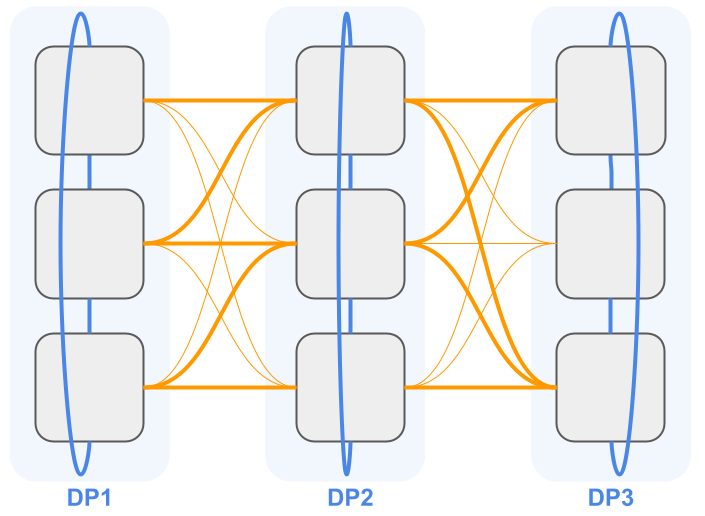
\includegraphics[width=0.45\textwidth]{figures/swarm.png}
  \caption{\textbf{SWARM Communication} We show high-level communication
  patterns in a 3x3 SWARM. SWARM interleaves PP and DP communication: First,
  activations take stochastic forward route through pipeline stages, gradients
  follow the same path backwards such that nodes accumulate gradients. Finally,
  gradients are averaged within stages via \texttt{AllReduce}.}
  \label{fig:swarm}
\end{figure}

% TODO: Add key observation of square-cube law
% -> DP communication scales cubic, PP communication only quadratic

\subsection{DiLoCo-SWARM}

One of two communication types in SWARM relies on costly gradient
synchronization between nodes in pipeline stages at every step. The success and
robustness of DiLoCo in replacing frequent gradient synchronization, motivates 
utilizing DiLoCo-like gradient synchronization, as described in
Algorithm~\ref{alg:diloco} as a drop-in replacement for regular gradient
synchronization within SWARM pipeline stages. We refer to this method as
DiLoCo-SWARM.

\section{Implementation}

% Question: Should I go in detail to explain the implementation?

% Introduction
A key contribution of this work is the release of the full experiment codebase
(\github{}) and a distilled single-file training script (\gist{}) which
implements all of the above mentioned distributed training methods in one place,
i.e. data, pipeline, and SWARM parallelism, with optional DiLoCo-style gradient
synchronization. Example invocations are shown in the Appendix.

% Advantages (Minimal, PyTorch-only, various algos, HF support)
The implementation is designed with simplicity and readability in mind. It only
depends on PyTorch, specifically the \texttt{torch.distributed} package, for
training and communication. Further, instead of multiple thousand lines of code 
of the original SWARM implementation, it uses only a few hundred. Put together,
this makes it easy for anybody to understand various traditional parallelization
techniques, and how they interact with decentralized variants, like DiLoCo and
SWARM. To enable quick testing and debugging, it can emulate nodes via threads.
Finally, it integrates with HuggingFace for models and datasets, allowing
diverse testing setups. In summary, we hope that the single-file training script
will be an excellent educational resource, and the full experiment codebase a
starting point for rapidly verifying and iterating on research ideas, as
showcased with DiLoCo-SWARM.

% Limitations (Not feature-complete and less efficient)
The simplicity comes at the cost of efficiency and feature-incompleteness. In
particular, a subset of SWARM features, most notably those enabling
fault-tolerance, are not yet supported. Some require features beyond what is
supported in PyTorch today. A full list of not-yet supported features is listed
in the Appendix. An important consequence of this is that the script currently
only supports runs on a single node with multiple workers, making the system
unusable in production-settings. Regardless, research is still possible, as, for
example, network latency can be artifically introduced to emulate a truly
decentral application. Finally, the training script does not use an advanced
scheduling technique for pipelining, and so time-to-accuracy comparison is not
meaningful.

% NanoGPT
The implementation should therefore be seen as a supplemental resource, focusing
on simplicity, and hackability. Our hope is that it might trigger a similar
effect as NanoGPT~\cite{karpathy2024nanogpt}, a minimal re-implementation of
GPT-2, which today serves as the default tool within the open-source community
to
benchmark research in deep learning components, such as architectures,
hyperparameters, or optimizers~\cite{moddednanogpt2024}.

\section{Experiments}

% Introduction
In this section we report the experiment setup and results validating
DiLoCo-SWARM. The setup and hyperparameters largely follow the
DiLoCo~\cite{douillard2023diloco} experiments.

% Dataset
We consider a language modeling task on the FineWeb-Edu~\cite{penedo2024fineweb}
dataset, a large pre-training dataset consisting of high-quality web pages
filtered for educational content. We choose this dataset over other common
pre-training datasets due to its high token efficiency allowing to match the
original GPT-2 performance on the
HellaSwag~\cite{zellers2019hellaswag} benchmark when training the same model with 10x
less data~\cite{karpathy2024nanogpt}.

% Model
For all experiments, we use the GPT-2 family of models~\cite{radford2019gpt2} which
are parameterized as shown in Table~\ref{tab:models}. Notice that the parameter 
counts slightly deviate from the original paper, since we do not share the 
weights of the embedding matrix and language modeling head to simplify training
in pipelined settings. Per default, we use GPT-2 Small and always train from 
randomly initialized models.

% Model sizes
\begin{table}[h]
\centering
\begin{tabular}{lcccc}
\toprule
\textbf{Model} & \textbf{Layers} & \textbf{Heads} & \textbf{Hidden Size} & \textbf{Params} \\
\midrule
Small & 12 & 12 & 768 & $\sim$180M \\
Medium & 24 & 16 & 1024 & $\sim$405M \\
Large & 36 & 20 & 1280 & $\sim$800M \\
\bottomrule
\end{tabular}
\caption{\textbf{Model Sizes.} GPT-2 model configurations used in experiments.
Parameter counts account for non-shared weights in embedding and language
modeling head.}
\label{tab:models}
\end{table}

% Hyper-parameters
The hyper-parameters are adapted from the tuning done in
DiLoCo~\cite{douillard2023diloco}: The default optimizer outer
AdamW~\cite{loshchilov2019adamw} with a learning rate of $4\cdot 10^{-4}$, and a
weight decay of $0.01$ which is linearly warmed up. When DiLoCo-style gradient
synchronization applies, we use a Nesterov with a learning rate of $0.7$ and a
momentum of $0.9$ as an global optimizer. A detailed description of the
hyperparameters is provided in Table~\ref{tab:hyperparameters} in the Appendix.

% Evaluation
Our main evaluation metric is the perplexity on a held-out validation set of 10M
randomly sampled tokens from FineWeb-Edu. We evaluate during and after training
to show the convergence against the number of training steps.

% Main Experiment: DiLoCo-SWARM
\textbf{Main Experiment.} Our main experiment setup closely follows that of
DiLoCo~\cite{douillard2023diloco}. We train two baselines and a DiLoCo-SWARM. The
\textit{weak baseline} trains for 2,000 steps on one GPU with a batch size of
512 and sequence length of 1024, for a total training budget of 1B tokens. The 
strong baseline is a 4x2 SWARM, i.e. eight workers distributed in two pipeline 
stages. This baseline performs regular gradient synchronization at every step.
The higher compute budget is used to scale the batch size to the number of
worker per stage, leading to a total training budget of 4B tokens. Finally, we
train a 4x2 DiLoCo-SWARM which uses the same setup and compute budget as the
strong baseline but performs the outer optimization step only every 50 steps.

\begin{figure*}[t]
  \centering
  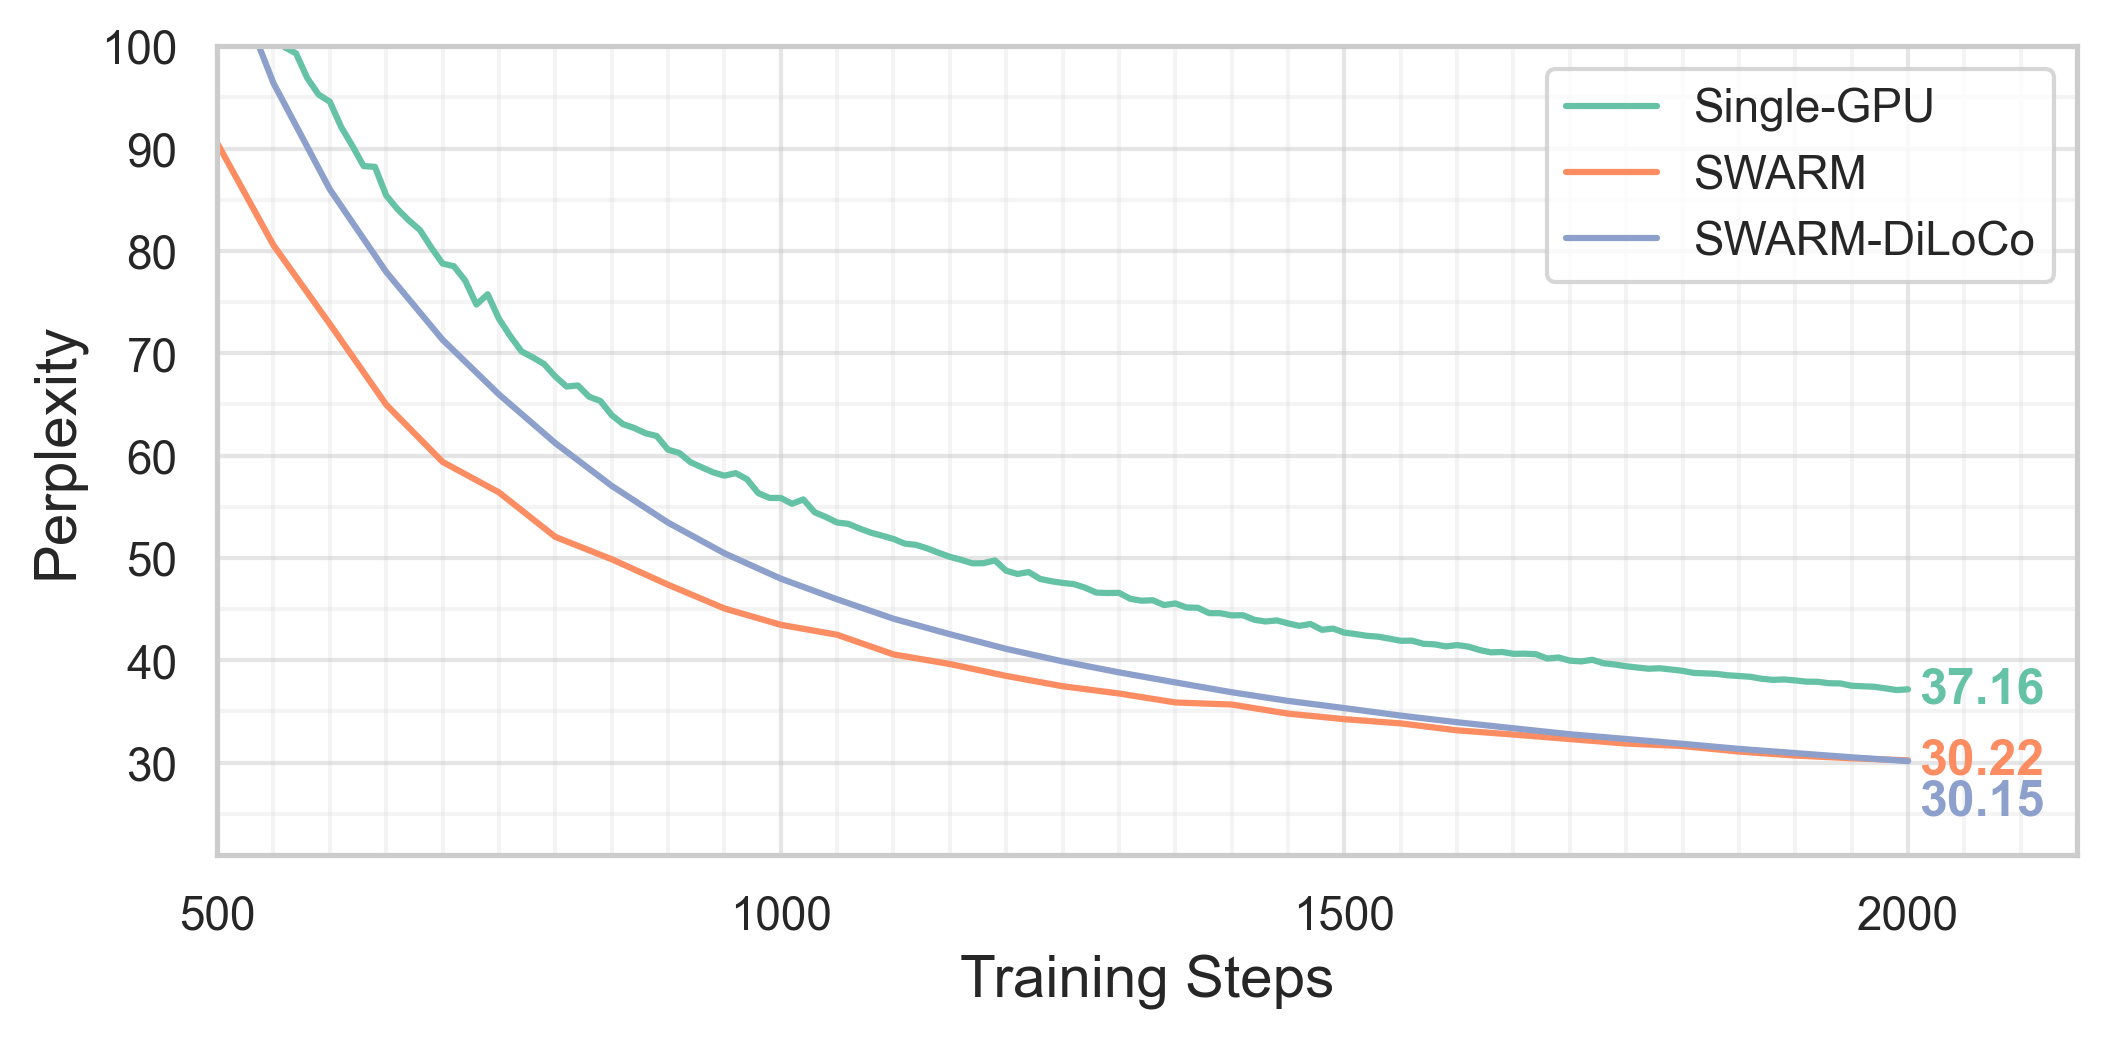
\includegraphics[width=0.8\textwidth]{figures/experiment1.png}
  \caption{\textbf{Main Result} We show the validation perplexity against the
  number of training steps for two baselines and SWARM-DiLoCo. With the same
  compute and data budget but with 50x less gradient synchronization,
  DiLoCo-SWARM matches the generalization performance of the strong SWARM
  baseline.}
  \label{fig:experiment1}
\end{figure*}

Figure~\ref{fig:experiment1} shows the validation perplexity as a function of
the training steps. Unsurprisingly, the weaker baseline, using less compute and
data, is outperformed by the stronger SWARM baseline with final perplexities of 
37.16 and 30.22, respectively. Our main finding is that DiLoCo-SWARM closely
matches, and even exceeds, the strong baseline in generalization performance
with a validation perplexity of 30.15, despite synchronizing gradients 50x fewer
times. This implies that DiLoCo-style gradient synchronization is compatible
with SWARM parallelism, allowing to reduce the communication cost incurred by 
gradient synchronization within pipeline stages of SWARM.

% Experiment 2: Ablation on communication frequency
\textbf{Communication Frequency.} We are interested in how \textit{infrequently}
gradient synchronization can occur within SWARM pipeline stages without
impacting convergence. Intuitively, the slower the frequency, the worse
convergence, but whether synchronizing every 10 or 200 steps negatively impacts
performance, has implications on the practical usefulness of the algorithm. To
investigate, we train five models using the same training setup and only vary
the number of local training steps before performing synchronizing gradients.

% TODO: Add perplexities in legend
% \begin{figure}[ht]
%   \centering
%   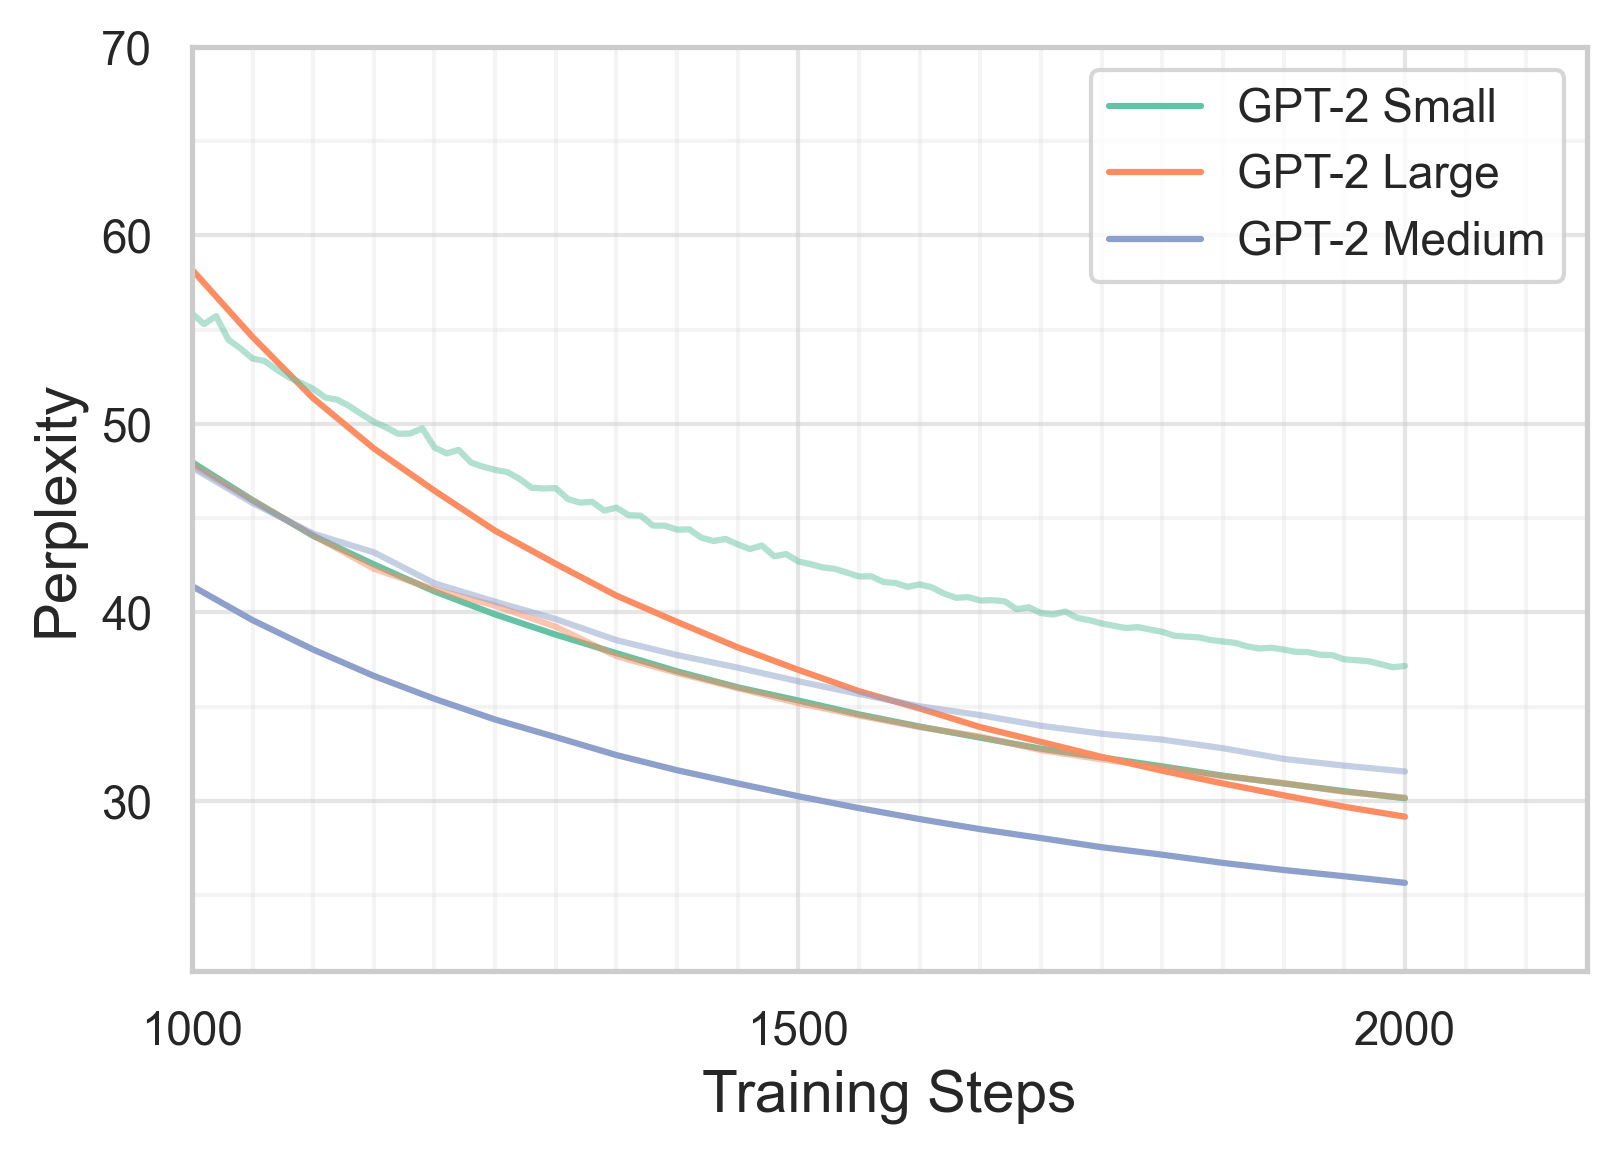
\includegraphics[width=0.45\textwidth]{figures/experiment3.png}
%   \caption{\textbf{Communication Frequency} We vary the number of local training
%   steps before performing an outer optimization step from $\{10, 20, 50, 100, 200\}$ 
%   and report the validation perplexity throughout training. Synchronizing more
%   frequently yields better results but performance degradation is neglibible even
%   on all tested values.}
%   \label{fig:experiment2}
% \end{figure}

Table~\ref{tab:experiment2} shows the results of this experiment. In line with
the original DiLoCo results, generalization performance monotonically increases
with higher gradient synchronization frequency. However, the performance
degradation for less frequent gradient synchronization is mild. Synchronizing
every 10 steps achieves the best performance, with a validation perplexity of
27.95. Note, that this also significantly out-performs the SWARM baseline in
Figure~\ref{fig:experiment1} while still reducing the synchronization frequency
by 10x. In our experiments, a good trade-off between communication frequency and
performance is achieved when synchronizing every 50 steps, which is therefore
used throughout all other experiments.

\begin{table}[ht]
\centering
\begin{tabular}{lccc}
\toprule
\textbf{Freq.} & \textbf{Val. PPL} & \textbf{$\Delta$ (Abs./Rel.)} \\ 
\midrule
10 & 27.95 & - \\
20 & 28.61 & 0.66 / 2.36\% \\
50 & 30.15 & 2.2 / 7.87\% \\
100 & 30.49 & 2.54 / 9.09\% \\
200 & 31.27 & 3.32 / 11.88\% \\
\bottomrule
\end{tabular}
\caption{\textbf{Communication Frequency} We report the final validation
perplexity for different communication frequencies and their absolute and
relative changes compared to synchronizing every 10 steps.}
\label{tab:experiment2}
\end{table}

% Experiment 3: Varying the model size
\textbf{Model Sizes.} Finally, we train three sizes of GPT-2 models, as 
described in Table~\ref{tab:models} to assess whether DiLoCo-style gradient
synchronization is robust scaling the model. We use the same hyper-parameters
for all models from Table~\ref{tab:hyperparameters} and train for 2,000 steps.
For each size, we also train a single-node baseline with four times smaller
batch size.

\begin{table}[ht]
\centering
\begin{tabular}{lccc}
\toprule
\textbf{\# Params} & \textbf{PPL} & \textbf{$\Delta$ (Abs./Rel.)} \\ 
\midrule
180M & 30.15 & 7.01 / 18.86\% \\
400M & 25.66 & 5.91 / 18.72\% \\
800M & & & \\
\bottomrule
\end{tabular}
\caption{\textbf{Model Size} We report the final validation perplexity for
different model sizes and their absolute and relative changes compared to a
single-node baseline with smaller batch size.}
\label{tab:experiment3}
\end{table}

Table~\ref{tab:experiment3} shows with DiLoCo we obtain a constant improvement
of $\sim$18\% over the single-node baseline run, for all tested model sizes.
This finding suggests that gradient synchronization with DiLoCo scales to larger
models sizes. This is an important finding as SWARM is designed to train models
which do not naively fit into a single nodes' memory and the scaling properties
of DiLoCo are hence crucial.

\section{Conclusion}

The results of this study suggest that DiLoCo-style gradient synchronization is
compatible with SWARM parallelism. This implies that gradient 
synchronization via a dual optimization scheme is an effective tool for gradient
synchronization, even when the gradients correspond to model shards in pipeline
stages accumulated via stochastic forward and backward passes.

These findings have implications both for the SWARM and DiLoCo community. For
SWARM, this means that the communication cost incurred by gradient
synchronization within pipeline stages can be drastically reduced. Hence, future
research and open-source efforts should focus on integrating DiLoCo-style 
gradient synchronization into production implementations of SWARM. For DiLoCo,
the findings further underline the robustness of the method, suggesting that
DiLoCo is a good candidate as a drop-in replacement anytime gradients need to be
synchronized between nodes in distributed settings.

\section{Limitations}

Several limitations to this work should be noted.

% Environment
All experiments were conducted on co-located GPUs with reliable and fast
interconnectivity. The initial premise of this research, however, was the
decentralized setting with unreliable, heterogeneous and poorly connected
compute resources. SWARM is only favourable over traditional parallelization
techniques in this setting, and so while the experiments in this study suggest
that DiLoCo-style gradient synchronization can be used in SWARM, it remains to
show how the method behaves in a truly decentral setting when scaled to larger
models, requiring more pipeline stages and nodes per stage.

% No tuning
Another limitation of this work is the lack of hyper-parameter tuning. All
hyper-parameters are copied from the tuned parameters in
DiLoCo~\cite{douillard2023diloco}. This might not always be fair, and lead to
pessimistic estimates of the validaiton performance. However, due to the
similarity of models, datasets, and training algorithms, we believe they are a
good proxy. Regardless, a sensible continuation of this work would be to
validate the results with tuned hyper-parameters.

% Scale
Moreover, it should be noted that the original DiLoCo and SWARM experiments were
conducted on larger scale. Both train on a data budget of roughly 50B tokens per
run, resulting in multiple GPU days worth of compute. Such resources were simply
not available within the scope of this project but is required to obtain robust
results on the efficacy of the algorithm.

% Efficiency
All of the above point to more more scale and compute. A crucial step is to
integrate optimized implementations of DiLoCo and SWARM, including efficient
pipeline scheduling techniques, allowing for fault-tolerant training over-the-
internt. Only then, experiments can be conducted on truly larger scale and in a
realistic environment. A particularly interesting question is how the reduced
communication frequency of gradients impacts the wall-clock runtime of the
algorithm in different network settings and for various model sizes.

% Different SWARM structures
Finally, another interesting, but open, research question is how the
DiLoCo-SWARM behaves when varying the number of workers per stage. The current
implementation does not scale beyond co-located GPUs, so investigating this
question requires implementing peer-to-peer communication over the Internet.

\section*{Acknowledgements}
\label{sec:acknowledgements}

This work was developed in collaboration with the Scalable Computing Systems
(SaCS) lab at EPFL as well as Prime Intellect. All compute was kindly sponsored
by Prime Intellect.

% Bibliography
\bibliography{references}
\bibliographystyle{icml2023}

% Appendix
\newpage
\appendix
\onecolumn

\section{Appendix}

% TODO: Supported and non-supported features in implementation

\subsection{Training Script Invocations}

Below we show example invocations for different distributed training algorithms.
All examples use a GPT-2 small model and the FineWeb-Edu dataset as an example.
For more details see the README on \github.

\begin{lstlisting}[language=bash]
# Single GPU training
torchrun --nproc_per_node 1 src/train.py --swarm.num_stages 1 \
    --model @configs/model/gpt2-small.toml \
    --data @configs/data/fineweb-edu-10bt.toml
\end{lstlisting}

\begin{lstlisting}[language=bash]
# Pipeline parallel training with 2 GPUs
torchrun --nproc_per_node 2 src/train.py --swarm.num_stages 2 \
    --model @configs/model/gpt2-small.toml \
    --data @configs/data/fineweb-edu-10bt.toml
\end{lstlisting}

\begin{lstlisting}[language=bash]
# Data parallel training with 2 GPUs
torchrun --nproc_per_node 2 src/train.py --swarm.num_stages 2 \
    --model @configs/model/gpt2-small.toml \
    --data @configs/data/fineweb-edu-10bt.toml
\end{lstlisting}

\begin{lstlisting}[language=bash]
# DiLoCo training with 2 GPUs
torchrun --nproc_per_node 2 src/train.py --swarm.num_stages 2 \
    --train.outer_optimizer @configs/optimizer/nesterov.toml
    --model @configs/model/gpt2-small.toml \
    --data @configs/data/fineweb-edu-10bt.toml
\end{lstlisting}

\begin{lstlisting}[language=bash]
# SWARM training with 4 GPUs
torchrun --nproc_per_node 4 src/train.py --swarm.num_stages 2 \
    --model @configs/model/gpt2-small.toml \
    --data @configs/data/fineweb-edu-10bt.toml
\end{lstlisting}

\begin{lstlisting}[language=bash]
# DiLoCo-SWARM training with 4 GPUs
torchrun --nproc_per_node 4 src/train.py --swarm.num_stages 2 \
    --train.outer_optimizer configs/optimizer/nesterov.toml
    --model @configs/model/gpt2-small.toml \
    --data @configs/data/fineweb-edu-10bt.toml
\end{lstlisting}

% Hyperparameters
\subsection{Hyperparameters}

Table~\ref{tab:hyperparameters} shows the hyperparameters used throughout the
experiments. The outer optimizer parameters is only used for DiLoCo-style
training, else the gradients are averaged before performing a regular optimizer
step by default.

\begin{table}[ht]
\centering
\begin{tabular}{llc}
\toprule
\textbf{Hyperparameter} & \textbf{Value} \\ 
\midrule
\multirow{1}{*}{General} & Batch Size & 512 \\ 
& Sequence Length & 1024 \\ 
& Steps & 2000 \\
\hline
\multirow{1}{*}{InnerOptimizer} & Name & AdamW \\ 
& Weight decay & - \\ 
& Learning Rate & $4 \times 10^{-4}$ \\ 
\hline
\multirow{1}{*}{OuterOptimizer} & Name & Nesterov \\ 
& Learning Rate & 0.7 \\ 
& Momentum & 0.9 \\ 
\bottomrule
\end{tabular}
\caption{Hyperparameters}
\label{tab:hyperparameters}
\end{table}

% Hardware
\subsection{Hardware}

All experiments were conducted on a single node with eight co-located H100 GPUs
on \href{https://app.primeintellect.com/}{Prime Intellect Compute}.

\end{document}